\documentclass{book}
\usepackage[a4paper,top=2.5cm,bottom=2.5cm,left=2.5cm,right=2.5cm]{geometry}
\usepackage{makeidx}
\usepackage{natbib}
\usepackage{graphicx}
\usepackage{multicol}
\usepackage{float}
\usepackage{listings}
\usepackage{color}
\usepackage{ifthen}
\usepackage[table]{xcolor}
\usepackage{textcomp}
\usepackage{alltt}
\usepackage{ifpdf}
\ifpdf
\usepackage[pdftex,
            pagebackref=true,
            colorlinks=true,
            linkcolor=blue,
            unicode
           ]{hyperref}
\else
\usepackage[ps2pdf,
            pagebackref=true,
            colorlinks=true,
            linkcolor=blue,
            unicode
           ]{hyperref}
\usepackage{pspicture}
\fi
\usepackage[utf8]{inputenc}
\usepackage[spanish]{babel}
\usepackage{mathptmx}
\usepackage[scaled=.90]{helvet}
\usepackage{courier}
\usepackage{sectsty}
\usepackage{amssymb}
\usepackage[titles]{tocloft}
\usepackage{doxygen}
\lstset{language=C++,inputencoding=utf8,basicstyle=\footnotesize,breaklines=true,breakatwhitespace=true,tabsize=2,numbers=left }
\makeindex
\setcounter{tocdepth}{3}
\renewcommand{\footrulewidth}{0.4pt}
\renewcommand{\familydefault}{\sfdefault}
\hfuzz=15pt
\setlength{\emergencystretch}{15pt}
\hbadness=750
\tolerance=750
\begin{document}
\hypersetup{pageanchor=false,citecolor=blue}
\begin{titlepage}
\vspace*{7cm}
\begin{center}
{\Large Laboratorio de P\-R\-O2. Ejercicio Gestión de una lavadora. \\[1ex]\large version 1 10-\/abr-\/2012 }\\
\vspace*{1cm}
{\large Generado por Doxygen 1.8.2}\\
\vspace*{0.5cm}
{\small Jueves, 10 de Abril de 2014 08:59:21}\\
\end{center}
\end{titlepage}
\clearemptydoublepage
\pagenumbering{roman}
\tableofcontents
\clearemptydoublepage
\pagenumbering{arabic}
\hypersetup{pageanchor=true,citecolor=blue}
\chapter{Ejemplo de diseño modular\-: Gestión de una lavadora.}
\label{index}\hypertarget{index}{}En este ejemplo se construye un programa modular que ofrece un menú de opciones para gestionar una lavadora. Se introducen las clases {\itshape \hyperlink{class_lavadora}{Lavadora}}, {\itshape \hyperlink{class_cubeta}{Cubeta}} y {\itshape \hyperlink{class_prenda}{Prenda}}. 
\chapter{Índice de clases}
\section{Lista de clases}
Lista de las clases, estructuras, uniones e interfaces con una breve descripción\-:\begin{DoxyCompactList}
\item\contentsline{section}{\hyperlink{class_cjt__organismes}{Cjt\-\_\-organismes} \\*Conté un conjunt d'organismes }{\pageref{class_cjt__organismes}}{}
\item\contentsline{section}{\hyperlink{class_organisme}{Organisme} \\*Contiene celulas ordenadas }{\pageref{class_organisme}}{}
\end{DoxyCompactList}

\chapter{Indice de archivos}
\section{Lista de archivos}
Lista de todos los archivos con descripciones breves\-:\begin{DoxyCompactList}
\item\contentsline{section}{\hyperlink{_lista_palabras_8hpp}{Lista\-Palabras.\-hpp} \\*Especificación de la clase \hyperlink{class_lista_palabras}{Lista\-Palabras} }{\pageref{_lista_palabras_8hpp}}{}
\item\contentsline{section}{\hyperlink{_palabra_8hpp}{Palabra.\-hpp} \\*Especificación de la clase \hyperlink{class_palabra}{Palabra} }{\pageref{_palabra_8hpp}}{}
\item\contentsline{section}{\hyperlink{pro2__s52_8cpp}{pro2\-\_\-s52.\-cpp} \\*Programa principal para el ejercicio {\itshape Factor Psi} }{\pageref{pro2__s52_8cpp}}{}
\end{DoxyCompactList}

\chapter{Documentación de las clases}
\hypertarget{class_cubeta}{\section{Referencia de la Clase Cubeta}
\label{class_cubeta}\index{Cubeta@{Cubeta}}
}


Representa una cubeta de ropa.  


\subsection*{Métodos públicos}
\begin{DoxyCompactItemize}
\item 
\hyperlink{class_cubeta_ae85e70c9cd67454446439891e3f435e1}{Cubeta} ()
\begin{DoxyCompactList}\small\item\em Creadora por defecto. \end{DoxyCompactList}\item 
\hyperlink{class_cubeta_a9615e48038899c5732f61661585f12c7}{Cubeta} (const \hyperlink{class_cubeta}{Cubeta} \&c)
\begin{DoxyCompactList}\small\item\em Creadora copiadora. \end{DoxyCompactList}\item 
void \hyperlink{class_cubeta_a431873df8f99cebe56b4787a5271e395}{anadir\-\_\-prenda} (const \hyperlink{class_prenda}{Prenda} \&p)
\begin{DoxyCompactList}\small\item\em Añade una prenda a la cubeta. \end{DoxyCompactList}\item 
void \hyperlink{class_cubeta_a3586257f2f2eacefc47714c6a3a01875}{completar\-\_\-lavadora} (\hyperlink{class_lavadora}{Lavadora} \&l)
\begin{DoxyCompactList}\small\item\em Completa una lavadora con las prendas de la cubeta. \end{DoxyCompactList}\item 
void \hyperlink{class_cubeta_a3448e45131b077516b3f12fe027642dd}{escribir\-\_\-cubeta} () const 
\begin{DoxyCompactList}\small\item\em Operación de escritura. \end{DoxyCompactList}\end{DoxyCompactItemize}


\subsection{Descripción detallada}
Representa una cubeta de ropa. 

Puede contener prendas blancas y de color. Puede usarse para intentar llenar una lavadora; en ese caso, las prendas se sacan de la cubeta en orden inverso al de entrada 

Definición en la línea 18 del archivo Cubeta.\-hpp.



\subsection{Documentación del constructor y destructor}
\hypertarget{class_cubeta_ae85e70c9cd67454446439891e3f435e1}{\index{Cubeta@{Cubeta}!Cubeta@{Cubeta}}
\index{Cubeta@{Cubeta}!Cubeta@{Cubeta}}
\subsubsection[{Cubeta}]{\setlength{\rightskip}{0pt plus 5cm}Cubeta\-::\-Cubeta (
\begin{DoxyParamCaption}
{}
\end{DoxyParamCaption}
)}}\label{class_cubeta_ae85e70c9cd67454446439891e3f435e1}


Creadora por defecto. 

Se ejecuta automáticamente al declarar una cubeta. \begin{DoxyPrecond}{Precondición}
cierto 
\end{DoxyPrecond}
\begin{DoxyPostcond}{Postcondición}
El resultado es una cubeta sin prendas de ningún tipo 
\end{DoxyPostcond}
\hypertarget{class_cubeta_a9615e48038899c5732f61661585f12c7}{\index{Cubeta@{Cubeta}!Cubeta@{Cubeta}}
\index{Cubeta@{Cubeta}!Cubeta@{Cubeta}}
\subsubsection[{Cubeta}]{\setlength{\rightskip}{0pt plus 5cm}Cubeta\-::\-Cubeta (
\begin{DoxyParamCaption}
\item[{const {\bf Cubeta} \&}]{c}
\end{DoxyParamCaption}
)}}\label{class_cubeta_a9615e48038899c5732f61661585f12c7}


Creadora copiadora. 

Permite declarar una cubeta nueva como copia de otra ya existente. \begin{DoxyPrecond}{Precondición}
cierto 
\end{DoxyPrecond}
\begin{DoxyPostcond}{Postcondición}
El resultado es una cubeta igual que c 
\end{DoxyPostcond}


\subsection{Documentación de las funciones miembro}
\hypertarget{class_cubeta_a431873df8f99cebe56b4787a5271e395}{\index{Cubeta@{Cubeta}!anadir\-\_\-prenda@{anadir\-\_\-prenda}}
\index{anadir\-\_\-prenda@{anadir\-\_\-prenda}!Cubeta@{Cubeta}}
\subsubsection[{anadir\-\_\-prenda}]{\setlength{\rightskip}{0pt plus 5cm}void Cubeta\-::anadir\-\_\-prenda (
\begin{DoxyParamCaption}
\item[{const {\bf Prenda} \&}]{p}
\end{DoxyParamCaption}
)}}\label{class_cubeta_a431873df8f99cebe56b4787a5271e395}


Añade una prenda a la cubeta. 

\begin{DoxyPrecond}{Precondición}
cierto 
\end{DoxyPrecond}
\begin{DoxyPostcond}{Postcondición}
El parámetro implícito pasa a contener sus prendas originales más p 
\end{DoxyPostcond}
\hypertarget{class_cubeta_a3586257f2f2eacefc47714c6a3a01875}{\index{Cubeta@{Cubeta}!completar\-\_\-lavadora@{completar\-\_\-lavadora}}
\index{completar\-\_\-lavadora@{completar\-\_\-lavadora}!Cubeta@{Cubeta}}
\subsubsection[{completar\-\_\-lavadora}]{\setlength{\rightskip}{0pt plus 5cm}void Cubeta\-::completar\-\_\-lavadora (
\begin{DoxyParamCaption}
\item[{{\bf Lavadora} \&}]{l}
\end{DoxyParamCaption}
)}}\label{class_cubeta_a3586257f2f2eacefc47714c6a3a01875}


Completa una lavadora con las prendas de la cubeta. 

\begin{DoxyPrecond}{Precondición}
l está inicializada 
\end{DoxyPrecond}
\begin{DoxyPostcond}{Postcondición}
Se han eliminado del parámetro implícito y se han añadido a l las prendas del parámetro implícito del color adecuado que más se acercan entre todas al peso máximo de l sin pasarse, elegiéndose primero las que se introdujeron en último lugar 
\end{DoxyPostcond}
\hypertarget{class_cubeta_a3448e45131b077516b3f12fe027642dd}{\index{Cubeta@{Cubeta}!escribir\-\_\-cubeta@{escribir\-\_\-cubeta}}
\index{escribir\-\_\-cubeta@{escribir\-\_\-cubeta}!Cubeta@{Cubeta}}
\subsubsection[{escribir\-\_\-cubeta}]{\setlength{\rightskip}{0pt plus 5cm}void Cubeta\-::escribir\-\_\-cubeta (
\begin{DoxyParamCaption}
{}
\end{DoxyParamCaption}
) const}}\label{class_cubeta_a3448e45131b077516b3f12fe027642dd}


Operación de escritura. 

\begin{DoxyPrecond}{Precondición}
cierto 
\end{DoxyPrecond}
\begin{DoxyPostcond}{Postcondición}
Escribe el contenido del parámetro implícito por el canal estándar de salida 
\end{DoxyPostcond}


La documentación para esta clase fue generada a partir del siguiente fichero\-:\begin{DoxyCompactItemize}
\item 
\hyperlink{_cubeta_8hpp}{Cubeta.\-hpp}\end{DoxyCompactItemize}

\hypertarget{class_lavadora}{\section{Referencia de la Clase Lavadora}
\label{class_lavadora}\index{Lavadora@{Lavadora}}
}


Representa una lavadora.  


\subsection*{Métodos públicos}
\begin{DoxyCompactItemize}
\item 
\hyperlink{class_lavadora_a2366b1cd0ba86f8ef8ba8504067dc114}{Lavadora} ()
\begin{DoxyCompactList}\small\item\em Creadora por defecto. \end{DoxyCompactList}\item 
void \hyperlink{class_lavadora_ad43871786bb680e22552103bc23adc71}{inicializar\-\_\-lavadora} (int pmax, bool col)
\begin{DoxyCompactList}\small\item\em Inicializa la lavadora. \end{DoxyCompactList}\item 
void \hyperlink{class_lavadora_a7e465e1f11ba5ba3cffcee1ce9507e79}{anadir\-\_\-prenda} (const \hyperlink{class_prenda}{Prenda} \&p)
\begin{DoxyCompactList}\small\item\em Añade una prenda a la lavadora. \end{DoxyCompactList}\item 
void \hyperlink{class_lavadora_a82bd403e688482030fcb95f0c3fd62d1}{lavado} ()
\begin{DoxyCompactList}\small\item\em Realiza un lavado. \end{DoxyCompactList}\item 
bool \hyperlink{class_lavadora_a0788f5869b65672123a0f53f278b6165}{esta\-\_\-inicializada} () const 
\begin{DoxyCompactList}\small\item\em Consultora del estado de la lavadora. \end{DoxyCompactList}\item 
bool \hyperlink{class_lavadora_a184836a74d8df69e21991c2873a613e1}{consultar\-\_\-color\-\_\-lavadora} () const 
\begin{DoxyCompactList}\small\item\em Consultora del color de la lavadora. \end{DoxyCompactList}\item 
int \hyperlink{class_lavadora_a0d04eefff885cb0f3e1462b2e85b2a99}{consultar\-\_\-peso\-\_\-lavadora} () const 
\begin{DoxyCompactList}\small\item\em Consultora del peso actual de la lavadora. \end{DoxyCompactList}\item 
int \hyperlink{class_lavadora_a9e687c3d38303e79ae5aea620d074a68}{consultar\-\_\-peso\-\_\-maximo} () const 
\begin{DoxyCompactList}\small\item\em Consultora del peso máximo de la lavadora. \end{DoxyCompactList}\item 
void \hyperlink{class_lavadora_a0794c20f7dbd5bbb545711ef8aec9978}{escribir\-\_\-lavadora} () const 
\begin{DoxyCompactList}\small\item\em Operación de escritura. \end{DoxyCompactList}\end{DoxyCompactItemize}


\subsection{Descripción detallada}
Representa una lavadora. 

Dispone de dos estados (inicializada / no inicializada); si está inicializada tiene un peso máximo y un color y admite depositar prendas de dicho color hasta alcanzar dicho peso máximo; si no está inicializada solo se puede inicializar 

Definición en la línea 16 del archivo Lavadora.\-hpp.



\subsection{Documentación del constructor y destructor}
\hypertarget{class_lavadora_a2366b1cd0ba86f8ef8ba8504067dc114}{\index{Lavadora@{Lavadora}!Lavadora@{Lavadora}}
\index{Lavadora@{Lavadora}!Lavadora@{Lavadora}}
\subsubsection[{Lavadora}]{\setlength{\rightskip}{0pt plus 5cm}Lavadora\-::\-Lavadora (
\begin{DoxyParamCaption}
{}
\end{DoxyParamCaption}
)}}\label{class_lavadora_a2366b1cd0ba86f8ef8ba8504067dc114}


Creadora por defecto. 

Se ejecuta automáticamente al declarar una lavadora. \begin{DoxyPrecond}{Precondición}
cierto 
\end{DoxyPrecond}
\begin{DoxyPostcond}{Postcondición}
El resultado es una lavadora no inicializada 
\end{DoxyPostcond}


\subsection{Documentación de las funciones miembro}
\hypertarget{class_lavadora_ad43871786bb680e22552103bc23adc71}{\index{Lavadora@{Lavadora}!inicializar\-\_\-lavadora@{inicializar\-\_\-lavadora}}
\index{inicializar\-\_\-lavadora@{inicializar\-\_\-lavadora}!Lavadora@{Lavadora}}
\subsubsection[{inicializar\-\_\-lavadora}]{\setlength{\rightskip}{0pt plus 5cm}void Lavadora\-::inicializar\-\_\-lavadora (
\begin{DoxyParamCaption}
\item[{int}]{pmax, }
\item[{bool}]{col}
\end{DoxyParamCaption}
)}}\label{class_lavadora_ad43871786bb680e22552103bc23adc71}


Inicializa la lavadora. 

\begin{DoxyPrecond}{Precondición}
El parámetro implícito no está inicializado, pmax$>$0 
\end{DoxyPrecond}
\begin{DoxyPostcond}{Postcondición}
El parámetro implícito pasa a estar inicializado con peso máximo \char`\"{}pmax\char`\"{} y color \char`\"{}col\char`\"{} 
\end{DoxyPostcond}
\hypertarget{class_lavadora_a7e465e1f11ba5ba3cffcee1ce9507e79}{\index{Lavadora@{Lavadora}!anadir\-\_\-prenda@{anadir\-\_\-prenda}}
\index{anadir\-\_\-prenda@{anadir\-\_\-prenda}!Lavadora@{Lavadora}}
\subsubsection[{anadir\-\_\-prenda}]{\setlength{\rightskip}{0pt plus 5cm}void Lavadora\-::anadir\-\_\-prenda (
\begin{DoxyParamCaption}
\item[{const {\bf Prenda} \&}]{p}
\end{DoxyParamCaption}
)}}\label{class_lavadora_a7e465e1f11ba5ba3cffcee1ce9507e79}


Añade una prenda a la lavadora. 

\begin{DoxyPrecond}{Precondición}
El parámetro implícito (L) está inicializado, color de p = color de L, peso de L + peso de p $<$= peso máximo de L; 
\end{DoxyPrecond}
\begin{DoxyPostcond}{Postcondición}
El parámetro implícito contiene su carga original más p 
\end{DoxyPostcond}
\hypertarget{class_lavadora_a82bd403e688482030fcb95f0c3fd62d1}{\index{Lavadora@{Lavadora}!lavado@{lavado}}
\index{lavado@{lavado}!Lavadora@{Lavadora}}
\subsubsection[{lavado}]{\setlength{\rightskip}{0pt plus 5cm}void Lavadora\-::lavado (
\begin{DoxyParamCaption}
{}
\end{DoxyParamCaption}
)}}\label{class_lavadora_a82bd403e688482030fcb95f0c3fd62d1}


Realiza un lavado. 

Representa que se realiza el lavado, se retiran la prendas que contiene la lavadora y ésta queda en estado de volver a usarse \begin{DoxyPrecond}{Precondición}
El parámetro implícito está inicializado, 
\end{DoxyPrecond}
\begin{DoxyPostcond}{Postcondición}
El parámetro implícito no está inicializado 
\end{DoxyPostcond}
\hypertarget{class_lavadora_a0788f5869b65672123a0f53f278b6165}{\index{Lavadora@{Lavadora}!esta\-\_\-inicializada@{esta\-\_\-inicializada}}
\index{esta\-\_\-inicializada@{esta\-\_\-inicializada}!Lavadora@{Lavadora}}
\subsubsection[{esta\-\_\-inicializada}]{\setlength{\rightskip}{0pt plus 5cm}bool Lavadora\-::esta\-\_\-inicializada (
\begin{DoxyParamCaption}
{}
\end{DoxyParamCaption}
) const}}\label{class_lavadora_a0788f5869b65672123a0f53f278b6165}


Consultora del estado de la lavadora. 

\begin{DoxyPrecond}{Precondición}
cierto 
\end{DoxyPrecond}
\begin{DoxyPostcond}{Postcondición}
El resultado indica si el parámetro implícito está inicializado 
\end{DoxyPostcond}
\hypertarget{class_lavadora_a184836a74d8df69e21991c2873a613e1}{\index{Lavadora@{Lavadora}!consultar\-\_\-color\-\_\-lavadora@{consultar\-\_\-color\-\_\-lavadora}}
\index{consultar\-\_\-color\-\_\-lavadora@{consultar\-\_\-color\-\_\-lavadora}!Lavadora@{Lavadora}}
\subsubsection[{consultar\-\_\-color\-\_\-lavadora}]{\setlength{\rightskip}{0pt plus 5cm}bool Lavadora\-::consultar\-\_\-color\-\_\-lavadora (
\begin{DoxyParamCaption}
{}
\end{DoxyParamCaption}
) const}}\label{class_lavadora_a184836a74d8df69e21991c2873a613e1}


Consultora del color de la lavadora. 

\begin{DoxyPrecond}{Precondición}
El parámetro implícito está inicializado 
\end{DoxyPrecond}
\begin{DoxyPostcond}{Postcondición}
El resultado es el color del parámetro implícito 
\end{DoxyPostcond}
\hypertarget{class_lavadora_a0d04eefff885cb0f3e1462b2e85b2a99}{\index{Lavadora@{Lavadora}!consultar\-\_\-peso\-\_\-lavadora@{consultar\-\_\-peso\-\_\-lavadora}}
\index{consultar\-\_\-peso\-\_\-lavadora@{consultar\-\_\-peso\-\_\-lavadora}!Lavadora@{Lavadora}}
\subsubsection[{consultar\-\_\-peso\-\_\-lavadora}]{\setlength{\rightskip}{0pt plus 5cm}int Lavadora\-::consultar\-\_\-peso\-\_\-lavadora (
\begin{DoxyParamCaption}
{}
\end{DoxyParamCaption}
) const}}\label{class_lavadora_a0d04eefff885cb0f3e1462b2e85b2a99}


Consultora del peso actual de la lavadora. 

\begin{DoxyPrecond}{Precondición}
El parámetro implícito está inicializado 
\end{DoxyPrecond}
\begin{DoxyPostcond}{Postcondición}
El resultado es la suma de los pesos de las prendas del parámetro implícito 
\end{DoxyPostcond}
\hypertarget{class_lavadora_a9e687c3d38303e79ae5aea620d074a68}{\index{Lavadora@{Lavadora}!consultar\-\_\-peso\-\_\-maximo@{consultar\-\_\-peso\-\_\-maximo}}
\index{consultar\-\_\-peso\-\_\-maximo@{consultar\-\_\-peso\-\_\-maximo}!Lavadora@{Lavadora}}
\subsubsection[{consultar\-\_\-peso\-\_\-maximo}]{\setlength{\rightskip}{0pt plus 5cm}int Lavadora\-::consultar\-\_\-peso\-\_\-maximo (
\begin{DoxyParamCaption}
{}
\end{DoxyParamCaption}
) const}}\label{class_lavadora_a9e687c3d38303e79ae5aea620d074a68}


Consultora del peso máximo de la lavadora. 

\begin{DoxyPrecond}{Precondición}
El parámetro implícito está inicializado 
\end{DoxyPrecond}
\begin{DoxyPostcond}{Postcondición}
El resultado es el peso máximo del parámetro implícito 
\end{DoxyPostcond}
\hypertarget{class_lavadora_a0794c20f7dbd5bbb545711ef8aec9978}{\index{Lavadora@{Lavadora}!escribir\-\_\-lavadora@{escribir\-\_\-lavadora}}
\index{escribir\-\_\-lavadora@{escribir\-\_\-lavadora}!Lavadora@{Lavadora}}
\subsubsection[{escribir\-\_\-lavadora}]{\setlength{\rightskip}{0pt plus 5cm}void Lavadora\-::escribir\-\_\-lavadora (
\begin{DoxyParamCaption}
{}
\end{DoxyParamCaption}
) const}}\label{class_lavadora_a0794c20f7dbd5bbb545711ef8aec9978}


Operación de escritura. 

\begin{DoxyPrecond}{Precondición}
El parámetro implícito está inicializado 
\end{DoxyPrecond}
\begin{DoxyPostcond}{Postcondición}
Escribe las propiedades y el contenido del parámetro implícito por el canal estándar de salida 
\end{DoxyPostcond}


La documentación para esta clase fue generada a partir del siguiente fichero\-:\begin{DoxyCompactItemize}
\item 
\hyperlink{_lavadora_8hpp}{Lavadora.\-hpp}\end{DoxyCompactItemize}

\hypertarget{class_prenda}{\section{Referencia de la Clase Prenda}
\label{class_prenda}\index{Prenda@{Prenda}}
}


Representa una prenda de ropa con atributos peso y color.  


\subsection*{Métodos públicos}
\begin{DoxyCompactItemize}
\item 
\hyperlink{class_prenda_adfd86b131c7f40c58b0cb4200eb55129}{Prenda} ()
\begin{DoxyCompactList}\small\item\em Creadora por defecto. \end{DoxyCompactList}\item 
\hyperlink{class_prenda_af15ff723083040b89bc495b4ec4b914e}{Prenda} (int pes, bool col)
\begin{DoxyCompactList}\small\item\em Creadora con valores concretos. \end{DoxyCompactList}\item 
void \hyperlink{class_prenda_a598bccf93cb8aa217a8533c0307c686f}{modificar\-\_\-prenda} (int pes, bool col)
\begin{DoxyCompactList}\small\item\em Modificadora de los atributos. \end{DoxyCompactList}\item 
int \hyperlink{class_prenda_ae886133326d46cc18dd9070d317a3ccb}{consul\-\_\-peso} () const 
\begin{DoxyCompactList}\small\item\em Consultora del peso. \end{DoxyCompactList}\item 
bool \hyperlink{class_prenda_a149632ba71127621c52917ef2e936c2e}{consul\-\_\-color} () const 
\begin{DoxyCompactList}\small\item\em Consultora del color. \end{DoxyCompactList}\item 
void \hyperlink{class_prenda_ab3bc4680187543b363088760533c7a07}{escribir\-\_\-prenda} () const 
\begin{DoxyCompactList}\small\item\em Operación de escritura. \end{DoxyCompactList}\end{DoxyCompactItemize}


\subsection{Descripción detallada}
Representa una prenda de ropa con atributos peso y color. 

Definición en la línea 13 del archivo Prenda.\-hpp.



\subsection{Documentación del constructor y destructor}
\hypertarget{class_prenda_adfd86b131c7f40c58b0cb4200eb55129}{\index{Prenda@{Prenda}!Prenda@{Prenda}}
\index{Prenda@{Prenda}!Prenda@{Prenda}}
\subsubsection[{Prenda}]{\setlength{\rightskip}{0pt plus 5cm}Prenda\-::\-Prenda (
\begin{DoxyParamCaption}
{}
\end{DoxyParamCaption}
)}}\label{class_prenda_adfd86b131c7f40c58b0cb4200eb55129}


Creadora por defecto. 

Se ejecuta automáticamente al declarar una prenda. \begin{DoxyPrecond}{Precondición}
cierto 
\end{DoxyPrecond}
\begin{DoxyPostcond}{Postcondición}
El resultado es una prenda sin valores determinados para sus atributos 
\end{DoxyPostcond}
\hypertarget{class_prenda_af15ff723083040b89bc495b4ec4b914e}{\index{Prenda@{Prenda}!Prenda@{Prenda}}
\index{Prenda@{Prenda}!Prenda@{Prenda}}
\subsubsection[{Prenda}]{\setlength{\rightskip}{0pt plus 5cm}Prenda\-::\-Prenda (
\begin{DoxyParamCaption}
\item[{int}]{pes, }
\item[{bool}]{col}
\end{DoxyParamCaption}
)}}\label{class_prenda_af15ff723083040b89bc495b4ec4b914e}


Creadora con valores concretos. 

\begin{DoxyPrecond}{Precondición}
pes$>$0 
\end{DoxyPrecond}
\begin{DoxyPostcond}{Postcondición}
El resultado es una prenda con peso \char`\"{}pes\char`\"{} y color \char`\"{}col\char`\"{} 
\end{DoxyPostcond}


\subsection{Documentación de las funciones miembro}
\hypertarget{class_prenda_a598bccf93cb8aa217a8533c0307c686f}{\index{Prenda@{Prenda}!modificar\-\_\-prenda@{modificar\-\_\-prenda}}
\index{modificar\-\_\-prenda@{modificar\-\_\-prenda}!Prenda@{Prenda}}
\subsubsection[{modificar\-\_\-prenda}]{\setlength{\rightskip}{0pt plus 5cm}void Prenda\-::modificar\-\_\-prenda (
\begin{DoxyParamCaption}
\item[{int}]{pes, }
\item[{bool}]{col}
\end{DoxyParamCaption}
)}}\label{class_prenda_a598bccf93cb8aa217a8533c0307c686f}


Modificadora de los atributos. 

\begin{DoxyPrecond}{Precondición}
pes$>$0 
\end{DoxyPrecond}
\begin{DoxyPostcond}{Postcondición}
El parámetro implícito pasa a tener peso \char`\"{}pes\char`\"{} y color \char`\"{}col\char`\"{} 
\end{DoxyPostcond}
\hypertarget{class_prenda_ae886133326d46cc18dd9070d317a3ccb}{\index{Prenda@{Prenda}!consul\-\_\-peso@{consul\-\_\-peso}}
\index{consul\-\_\-peso@{consul\-\_\-peso}!Prenda@{Prenda}}
\subsubsection[{consul\-\_\-peso}]{\setlength{\rightskip}{0pt plus 5cm}int Prenda\-::consul\-\_\-peso (
\begin{DoxyParamCaption}
{}
\end{DoxyParamCaption}
) const}}\label{class_prenda_ae886133326d46cc18dd9070d317a3ccb}


Consultora del peso. 

\begin{DoxyPrecond}{Precondición}
cierto 
\end{DoxyPrecond}
\begin{DoxyPostcond}{Postcondición}
El resultado es el peso del parámetro implícito 
\end{DoxyPostcond}
\hypertarget{class_prenda_a149632ba71127621c52917ef2e936c2e}{\index{Prenda@{Prenda}!consul\-\_\-color@{consul\-\_\-color}}
\index{consul\-\_\-color@{consul\-\_\-color}!Prenda@{Prenda}}
\subsubsection[{consul\-\_\-color}]{\setlength{\rightskip}{0pt plus 5cm}bool Prenda\-::consul\-\_\-color (
\begin{DoxyParamCaption}
{}
\end{DoxyParamCaption}
) const}}\label{class_prenda_a149632ba71127621c52917ef2e936c2e}


Consultora del color. 

\begin{DoxyPrecond}{Precondición}
cierto 
\end{DoxyPrecond}
\begin{DoxyPostcond}{Postcondición}
El resultado es el color del parámetro implícito 
\end{DoxyPostcond}
\hypertarget{class_prenda_ab3bc4680187543b363088760533c7a07}{\index{Prenda@{Prenda}!escribir\-\_\-prenda@{escribir\-\_\-prenda}}
\index{escribir\-\_\-prenda@{escribir\-\_\-prenda}!Prenda@{Prenda}}
\subsubsection[{escribir\-\_\-prenda}]{\setlength{\rightskip}{0pt plus 5cm}void Prenda\-::escribir\-\_\-prenda (
\begin{DoxyParamCaption}
{}
\end{DoxyParamCaption}
) const}}\label{class_prenda_ab3bc4680187543b363088760533c7a07}


Operación de escritura. 

\begin{DoxyPrecond}{Precondición}
cierto 
\end{DoxyPrecond}
\begin{DoxyPostcond}{Postcondición}
Se han escrito los atributos del parámetro implícito en el canal standard de salida. 
\end{DoxyPostcond}


La documentación para esta clase fue generada a partir del siguiente fichero\-:\begin{DoxyCompactItemize}
\item 
\hyperlink{_prenda_8hpp}{Prenda.\-hpp}\end{DoxyCompactItemize}

\chapter{Documentación de archivos}
\hypertarget{_cubeta_8hpp}{\section{Referencia del Archivo Cubeta.\-hpp}
\label{_cubeta_8hpp}\index{Cubeta.\-hpp@{Cubeta.\-hpp}}
}


Especificación de la clase \hyperlink{class_cubeta}{Cubeta}.  


Dependencia gráfica adjunta para Cubeta.\-hpp\-:
\nopagebreak
\begin{figure}[H]
\begin{center}
\leavevmode
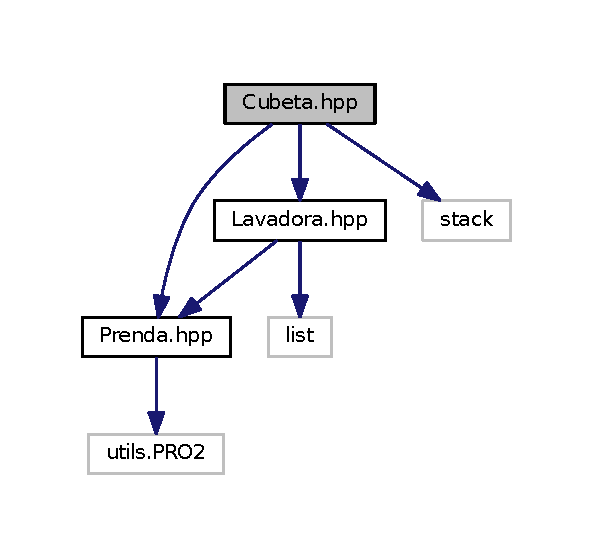
\includegraphics[width=284pt]{_cubeta_8hpp__incl}
\end{center}
\end{figure}
\subsection*{Clases}
\begin{DoxyCompactItemize}
\item 
class \hyperlink{class_cubeta}{Cubeta}
\begin{DoxyCompactList}\small\item\em Representa una cubeta de ropa. \end{DoxyCompactList}\end{DoxyCompactItemize}


\subsection{Descripción detallada}
Especificación de la clase \hyperlink{class_cubeta}{Cubeta}. 

Definición en el archivo \hyperlink{_cubeta_8hpp_source}{Cubeta.\-hpp}.


\hypertarget{_lavadora_8hpp}{\section{Referencia del Archivo Lavadora.\-hpp}
\label{_lavadora_8hpp}\index{Lavadora.\-hpp@{Lavadora.\-hpp}}
}


Especificación de la clase \hyperlink{class_lavadora}{Lavadora}.  


Dependencia gráfica adjunta para Lavadora.\-hpp\-:
\nopagebreak
\begin{figure}[H]
\begin{center}
\leavevmode
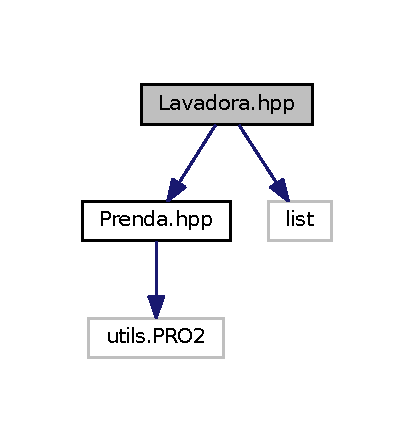
\includegraphics[width=198pt]{_lavadora_8hpp__incl}
\end{center}
\end{figure}
\subsection*{Clases}
\begin{DoxyCompactItemize}
\item 
class \hyperlink{class_lavadora}{Lavadora}
\begin{DoxyCompactList}\small\item\em Representa una lavadora. \end{DoxyCompactList}\end{DoxyCompactItemize}


\subsection{Descripción detallada}
Especificación de la clase \hyperlink{class_lavadora}{Lavadora}. 

Definición en el archivo \hyperlink{_lavadora_8hpp_source}{Lavadora.\-hpp}.


\hypertarget{_prenda_8hpp}{\section{Referencia del Archivo Prenda.\-hpp}
\label{_prenda_8hpp}\index{Prenda.\-hpp@{Prenda.\-hpp}}
}


Especificación de la clase \hyperlink{class_prenda}{Prenda}.  


Dependencia gráfica adjunta para Prenda.\-hpp\-:\nopagebreak
\begin{figure}[H]
\begin{center}
\leavevmode
\includegraphics[width=150pt]{_prenda_8hpp__incl}
\end{center}
\end{figure}
\subsection*{Clases}
\begin{DoxyCompactItemize}
\item 
class \hyperlink{class_prenda}{Prenda}
\begin{DoxyCompactList}\small\item\em Representa una prenda de ropa con atributos peso y color. \end{DoxyCompactList}\end{DoxyCompactItemize}


\subsection{Descripción detallada}
Especificación de la clase \hyperlink{class_prenda}{Prenda}. 

Definición en el archivo \hyperlink{_prenda_8hpp_source}{Prenda.\-hpp}.


\hypertarget{pro2__s8_8cpp}{\section{Referencia del Archivo pro2\-\_\-s8.\-cpp}
\label{pro2__s8_8cpp}\index{pro2\-\_\-s8.\-cpp@{pro2\-\_\-s8.\-cpp}}
}
Dependencia gráfica adjunta para pro2\-\_\-s8.\-cpp\-:
\nopagebreak
\begin{figure}[H]
\begin{center}
\leavevmode
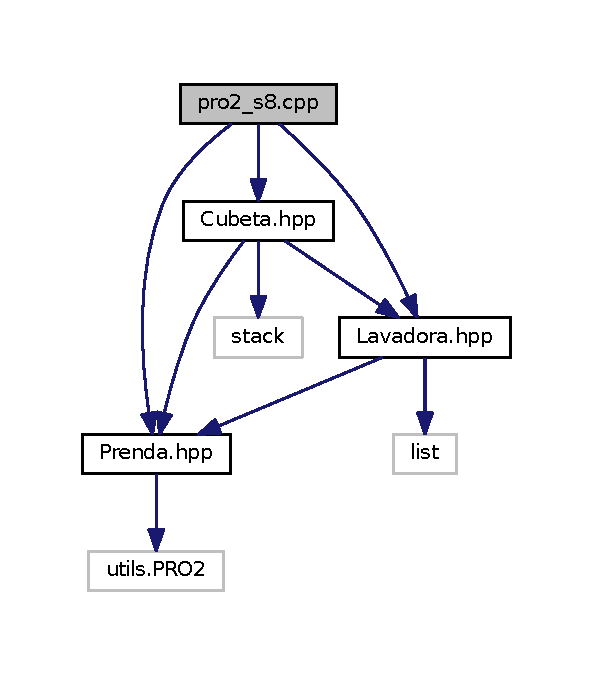
\includegraphics[width=285pt]{pro2__s8_8cpp__incl}
\end{center}
\end{figure}
\subsection*{Funciones}
\begin{DoxyCompactItemize}
\item 
int \hyperlink{pro2__s8_8cpp_ae66f6b31b5ad750f1fe042a706a4e3d4}{main} ()
\begin{DoxyCompactList}\small\item\em Programa principal para el ejercicio {\itshape Gestión de una lavadora}. \end{DoxyCompactList}\end{DoxyCompactItemize}


\subsection{Documentación de las funciones}
\hypertarget{pro2__s8_8cpp_ae66f6b31b5ad750f1fe042a706a4e3d4}{\index{pro2\-\_\-s8.\-cpp@{pro2\-\_\-s8.\-cpp}!main@{main}}
\index{main@{main}!pro2_s8.cpp@{pro2\-\_\-s8.\-cpp}}
\subsubsection[{main}]{\setlength{\rightskip}{0pt plus 5cm}int main (
\begin{DoxyParamCaption}
{}
\end{DoxyParamCaption}
)}}\label{pro2__s8_8cpp_ae66f6b31b5ad750f1fe042a706a4e3d4}


Programa principal para el ejercicio {\itshape Gestión de una lavadora}. 



Definición en la línea 20 del archivo pro2\-\_\-s8.\-cpp.


\begin{DoxyCode}
\{
    \hyperlink{class_lavadora}{Lavadora} Lav;
    \hyperlink{class_cubeta}{Cubeta} Cubet;
    \textcolor{keywordtype}{int} x=readint();
    \textcolor{keywordflow}{while} (x != -8)\{
        \textcolor{keywordflow}{if} (x == -1)\{
            cout << \textcolor{stringliteral}{"peso: "};
            \textcolor{keywordtype}{int} peso=readint();
            cout << endl << \textcolor{stringliteral}{"color: B blanco, Otro Color: "};
            \textcolor{keywordtype}{char} color=readchar();
            cout << endl;
            \textcolor{keywordtype}{bool} p=\textcolor{keyword}{true};
            \textcolor{keywordflow}{if} (color==\textcolor{charliteral}{'B'}) p=\textcolor{keyword}{false};
            Lav.\hyperlink{class_lavadora_ad43871786bb680e22552103bc23adc71}{inicializar\_lavadora}(peso,p);
            cout << \textcolor{stringliteral}{"lavadora inicializada"} << endl;
        \}
        \textcolor{keywordflow}{if} (x == -2)\{
            cout << \textcolor{stringliteral}{"peso: "};
            \textcolor{keywordtype}{int} peso=readint();
            cout << endl << \textcolor{stringliteral}{"color: B blanco, Otro Color: "};
            \textcolor{keywordtype}{char} color=readchar();
            cout << endl;
            \textcolor{keywordtype}{bool} p=\textcolor{keyword}{true};
            \textcolor{keywordflow}{if} (color==\textcolor{charliteral}{'B'}) p=\textcolor{keyword}{false};
            \hyperlink{class_prenda}{Prenda} Prend(peso,p);
            Lav.\hyperlink{class_lavadora_a7e465e1f11ba5ba3cffcee1ce9507e79}{anadir\_prenda}(Prend);
        \}
        \textcolor{keywordflow}{if} (x == -3)\{
            cout << \textcolor{stringliteral}{"peso: "};
            \textcolor{keywordtype}{int} peso=readint();
            cout << endl << \textcolor{stringliteral}{"color: B blanco, Otro Color: "};
            \textcolor{keywordtype}{char} color=readchar();
            cout << endl;
            \textcolor{keywordtype}{bool} p=\textcolor{keyword}{true};
            \textcolor{keywordflow}{if} (color==\textcolor{charliteral}{'B'}) p=\textcolor{keyword}{false};
            \hyperlink{class_prenda}{Prenda} Prend(peso,p);
            Cubet.\hyperlink{class_cubeta_a431873df8f99cebe56b4787a5271e395}{anadir\_prenda}(Prend);
        \}
        \textcolor{keywordflow}{if} (x == -4)\{
            Cubet.\hyperlink{class_cubeta_a3586257f2f2eacefc47714c6a3a01875}{completar\_lavadora}(Lav);
        \}
        \textcolor{keywordflow}{if} (x == -5)\{
            Lav.\hyperlink{class_lavadora_a82bd403e688482030fcb95f0c3fd62d1}{lavado}();
        \}
        \textcolor{keywordflow}{if} (x == -6)\{
            Cubet.\hyperlink{class_cubeta_a3448e45131b077516b3f12fe027642dd}{escribir\_cubeta}();
        \}
        \textcolor{keywordflow}{if} (x==-7)\{
            Lav.\hyperlink{class_lavadora_a0794c20f7dbd5bbb545711ef8aec9978}{escribir\_lavadora}();
        \}
        x=readint();
    \}
    cout << \textcolor{stringliteral}{"fin"} << endl;

\}
\end{DoxyCode}

\addcontentsline{toc}{part}{Índice}
\printindex
\end{document}
